% !TEX TS-program = pdflatex
\newif\ifresearch
\researchtrue % comment out to hide answers


\newif\iftwopage
\twopagetrue % comment this out to keep resume to two pages


\documentclass{article}
\pagenumbering{gobble}
\usepackage[raggedright]{titlesec}
\usepackage{etoolbox}
\usepackage{mfirstuc}	
\usepackage{hyperref}
\usepackage{titling}
\usepackage{amsmath}
\usepackage[margin=0.5in]{geometry}
\usepackage{array}
\usepackage{tabu}
\usepackage{multirow}
\usepackage{longtable}
\usepackage[utf8]{inputenc}
\usepackage{fancyhdr}
\usepackage{graphicx}
\usepackage{blindtext}
\usepackage{wrapfig}
\usepackage{enumitem}
\setlist{nosep}

\setlength{\arrayrulewidth}{0.05mm}

\titleformat{\section}[leftmargin]
{\raggedright\scshape\titlerule\vspace{0.5ex}}
{}
{0pt}
{}
\titlespacing*{\section}{2.8cm}{*1.8}{0.1cm}

\newcommand{\mygeometry}[1]{%
  \geometry{right=#1,left=\dimexpr#1+20mm\relax}
}
\mygeometry{15mm}

\titleformat{\subsubsection}[runin]
{\vspace{0.5ex}}
{$\bullet$}
{0.5em}
{}

\titlespacing{\subsubsection}
{0em}{0.1em}{1em}

\hypersetup{
    colorlinks=true,
    linkcolor=blue,
    filecolor=magenta,      
    urlcolor=cyan,
}
 
\urlstyle{same}

\title{Resume}
\date{2017-06-17}
\author{Abhishek Vaid}	

\begin{document}
\begin{huge} 
	\noindent Abhishek Vaid \hspace{1ex}
\end{huge} \href{http://linkedin.com/in/vaidabhishek86}{
\includegraphics[height=4ex]{linkedin}}
\hspace{4ex} \href{https://twitter.com/vaidabhishek}{
\includegraphics[height=4ex]{twitter}}
\hspace{3ex} \href{https://angel.co/abhishek-vaid}{
\includegraphics[height=4ex]{angellist}}\\
\noindent \href{mailto: vaid.abhi@gmail.com}{vaid.abhi@gmail.com} \\+91 (0)9886052252\\   
\vspace{-95pt}
\begin{flushright}
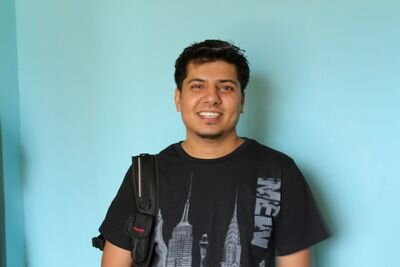
\includegraphics[width=3.0cm]{vaid}
\end{flushright}
 \vspace{-15pt}
\section{Profile}

\ifresearch
A former \textbf{entrepreneur} who is extremely passionate about intersection of \textbf{Technology, Software and Business}. I'm currently working as a \textbf{Technical Architect} at \href{https://www.urbancompany.com}{Urban Company}, Gurgram, India, where I contribute to consumer growth vertical by designing, architecting, optimizing and maintaining software frameworks and allied implementations. Before this, I worked as a \textbf{Co-Founder} and \textbf{Chief Architect} at \href{http://www.frrole.ai}{Frrole AI} --- A Bangalore based startup and an \textbf{AI platform that analyzes large scale social data streams to power interesting consumer intelligence use-cases}. I have adequate hands-on experience and deep interest in disciplines like \textbf{Large scale Software Implementations, Machine Learning, Data Science and design/implementation of Data driven Platforms}. Before Frrole, I was engaged in various teaching positions, contributed to multiple academic projects and have published several research papers. I am a strong advocate of continuous self-driven growth and therefore an active participant on leading self-learning platforms like \textbf{edX, Coursera, Udacity, FutureLearn and CognitiveClass.ai}. On average, I spend anywhere between \textbf{10 to 15 hours per week} on these platforms to learn new technologies.
\else

A post-graduate engineer, computer science enthusiast and a startup guy.  

\fi

\section{Education}
\begin{itemize}[leftmargin=-0.1ex]\setlength\itemsep{0.25em}\vspace{-10pt}
  \item[]  \href{http://iiitm.ac.in}{Indian Institute of Information Technology and Management (IIITM), Gwalior} \hfill Madhya Pradesh, India
  \item[] \textbf{5 Year Integrated Post Graduation in Information Technology} (CGPA: \textbf{8.34 /10}) \hfill 2004--2009
\end{itemize}\vspace{-3pt}

\section{Interests}
\begin{itemize}[leftmargin=-0.1ex]\setlength\itemsep{0.25em}\vspace{-10pt}
  \item Algorithm Design and Data Structures
  \item Machine Learning, NLP, Text Mining
  \item Data Science and Large Scale Data Processing
  \item Distributed and Parallel Processing Systems
  \item Software Architecture and Design Patterns
\end{itemize}\vspace{-3pt}

\section{Hands-On Skills }
\begin{itemize}[leftmargin=-0.1ex]\setlength\itemsep{0.25em}\vspace{-10pt}
  \item \textbf{Programming languages}: Python, Java, Javascript, Python, C++,  Scala, ML, Racket, Ruby, GoLang and Rust (basics)
  \item \textbf{Distributed Processing Frameworks}: Apache Storm, Apache Spark (basics), Apache Hadoop 2.0 (basics)
   \item \textbf{Databases}: MongoDB, Elasticsearch, MySQL, PostgreSql, Redis
   \item \textbf{Cloud Platforms}: AWS, Google Cloud, Microsoft Azure
\end{itemize}\vspace{-3pt}
  
\section{Work Profile}


\begin{itemize}[leftmargin=-1ex] \setlength\itemsep{0.25em}\vspace{5pt}
	
	
	\item[09/18' – Present] \href{https://urbanclap.com/}{\textbf{UrbanClap Technologies}} \textbf{Technical Architect}\hfill Bengaluru, India
	
	\item[]  \textbf{Urban Company} --- Urban Company (UC) is a Gurugram (India) based startup currently disrupting and redefining the online home services domain. Currently, UC is the market leader in India and has presence is 3 more countries. At UC, I own the entire backend engineering for consumer growth. This includes, having to engage with product, business and other engineering heads to chartout a roadmap and governing its healthy execution. Through my years I've managed teams of various sizes including people with varied experience levels. \vspace{5pt}
	
	\begin{itemize} \setlength\itemsep{0.5em}
		
		\item \href{https://urbanclap.com/weddings} {UC Homes/Weddings Content-Portal} - A content-rich and navigationally deep discovery platform. \\ I handled the end-to-end execution of the backend from scratch. The project took around 8 weeks. The portal supports billions of SEO friendly navigational links and houses 200K+ photos across two categories: \href{https://urbanclap.com/homes} {UC Homes} and \href{https://urbanclap.com/weddings} {UC Weddings}. The backend also supports the concept of Ideabook, where a user can curate his/her photos.
		\item {Logging and ELK Stack} - Architected and implemented Elastic Stack and Logging Funnel. 100 GB / day of system and event logs are being indexed coming from more than 20 micro-services. Deployed a full-scale ELK cluster to support this workload and published libraries for instantiating internal logging funnel across a suite of micro-services. The project was completed in 6 weeks. 
		\item {Core SEO API suite} - Designed and implemented a new API stack to power UC's SEO use-case. Because of this effort, UC enjoyed top positions in 1st page search results for most of the competitive categories in the business. 
		\item {Delivery and Pricing  Engine} - Architected and implemented a core sub-system to power pricing logic throughout the platform. The challenge here was to model things in a way that it becomes sufficiently easy for business and product owners to experiment and plug complex business rules to power complex pricing logic. This system powers the current UC pricing logic in several categories. 
		\item {Surge and Advance Payment} - Designed and Implemented Surge and Advance Payment construct on our consumer app. This project again requires good modeling to aid complex rules to derive on-they-fly surge signals to affect dynamic and real-time pricing based on demand / supply equivalence.
		\item {Refactoring} - As the only architect at UC, I took key refactoring projects to kill debt and facilitate our micr-service architecture.  
	\end{itemize}\vspace{5pt}
	
  \item[12/12' – 07/17'] \href{https://frrole.ai/}{\textbf{Frrole AI:}} \textbf{Co-founder and Chief Architect}\hfill Bengaluru, India
  \item[]  \textbf{Frrole AI} --- A Bangalore based \textbf{global AI Start-Up} that is redefining consumer intelligence by deploying best-in-class \textbf{AI and Machine Learning technologies to real-time large-scale social datasets from multiple networks}. I was involved in defining and shaping all aspects of Frrole ranging from \textbf{software architecture to design, development and scaling of our technical infrastructure}. I was also responsible for hiring and setting up our core team. 
  
From a technical standpoint, here are some of the projects that I worked on:  \vspace{5pt}
  
  	\begin{itemize} \setlength\itemsep{0.5em}
    
    \item \href{https://frrole.ai/deepsense}{Frrole DeepSense} - An innovative and novel offering that \textbf{builds the personality profile and preference models of a potential customer based on their publicly available social footprint}. The platform also engineers predictive attributes about a person's behavior, needs, demographics and possible choices.
  
 	\item \href{https://frrole.ai/platform}{Frrole Consumer Intelligence Platform} - A suite of business-ready intelligence applications comprising of \href{http://api.frrole.com/}{Frrole Intelligence APIs} and \href{https://frrole.ai/scout}{Frrole Scout}. The product processes over 50 million data points every day in real-time to provide live api feed to over 30+ clients. The platform also provides historical access to over 20 TB of curated data. 
  
  	\item \textbf{Frrole News} - An \textbf{autonomous news aggregation engine} powered by real-time analysis of social data streamed from Twitter at a large scale. I designed, developed and scaled the core backend data models, APIs and intelligence layer. 
  	
	\end{itemize}
     
   \item[08/09' – 04/12'] \textbf{Head-Coordinator} and \textbf{Lecturer} at LPU \hfill Jalandhar, India
   
   \item[] I was responsible for managing the entire department comprising of \textbf{28 faculty members and 500 enrolled students}. I was directly responsible for \textbf{teaching quality}, \textbf{curriculum design}, and \textbf{pedagogical innovations}. I also \textbf{designed} and \textbf{instructed courses} on subjects like Data Mining, Distributed Systems, Data Structures, Linux, OOPS, Multimedia Communication, Java Programming, and Algorithms.

\end{itemize}

\begin{itemize}[leftmargin=-1ex] \setlength\itemsep{0.25em}
    \item[05/12' – 12/12'] \textbf{Learning Break} \hfill New Delhi, India
   \item[] Took a study break to augment my knowledge and enhance my skill set by pursuing relevant coursework (MOOC- Massively Open Online Courses) on platforms like \textbf{Coursera}, \textbf{edX}, and \textbf{Udacity}. Overall, I completed \textbf{22+ certified courses} in 8 months.
%  \item[05/08' – 07/08'] \textbf{Summer Intern at Sunworks Consultants Pvt. Ltd.} \hfill Gurugram, India
%   \item[] Conducted preliminary analysis in the field of Threat Assessment and Risk Evaluation, followed by the development of algorithms and strategies to fuel an Autonomous System for Threat Assessment and Evaluation.
\end{itemize}

\section{Projects}
\begin{itemize}[leftmargin=-1ex]\setlength\itemsep{0.25em}\vspace{5pt}
   \item[08/08' – 08/09'] Master Thesis  --- \textbf{``Performance Analysis of Novel Evolutionary Algorithm Operators: An Implementation On Bounded Diameter Spanning Tree Problem''}. The research results were subsequently published in Proceedings of International Conference on Contemporary Computing.
    \item[01/09' – 06/09'] \textbf{``Knowledge Discovery in Databases Using Evolutionary Algorithms''}, to understand the strengths \& weaknesses of using Multi-Objective Evolutionary Algorithms to solve association rule mining problems.
   \item[07/08' – 08/08']  Developed an AI technique based on \textbf{Self Organizing Feature Maps} to automate the task of question selection in generating automatic online Question Paper Sets for various competitive examinations.
  %\item[05/07' – 08/07'] Bachelor's Thesis --- Developed \textbf{``FePAT - Fuzzy enabled Personality Assessment Technique''},  a  framework to maintain large-scale personality inventories for web applications. The whole framework and its core model were \textbf{tested with real world data} collected using custom made Fuzzy Based Questionnaire. 
   %\item[07/07' – 04/08'] Worked to mine out important \textbf{Multi-Dimensional Association Rules} from an \textbf{Environmental Dataset} of over 4 million records collected from over 30 sites in India. Algorithms were coded in Java.
\end{itemize}

\section{Some \\ Publications}
\begin{itemize}[leftmargin=-1ex]\setlength\itemsep{0.25em}\vspace{-10pt}
\item \textbf{``Association Rule Mining Using Multi-objective Genetic Algorithms: Strengths and Challenges''} presented at World Congress on Nature and Biologically Inspired Computing, 2009, Coimbatore. 
\item \textbf{``Multidimensional Association Rules from Large Weather Data Set: A Proposed Methodology''} accepted in Proceedings of International Conference on  Data Mining (DMIN), 2008, Las Vegas, USA. 
\item \textbf{``Automated Question Selection for Online Tests: A Novel Approach''} presented at International Congress on Pervasive Computing \& Management, 2008, New Delhi, India. 
%\item \textbf{``A Fuzzy enabled Personality Assessment Technique: FePAT''} presented at International Conference on Statistics and its Applications in Management (ICSAIM), 2008,  IIM Kozhikode, India.
%\item Paper based on my Master's Thesis: \textbf{``Property Analysis and Enhancement in Recombination Operator of Edge-Set Encoding for Spanning Tree Problem''}  presented at International Conference on Contemporary Computing (IC3),  2011, Noida, India.\label{masterthesis}
\end{itemize}
	
\section{Self \\  Learning }
\begin{itemize}[leftmargin=-1ex]\setlength\itemsep{0.25em}\vspace{-10pt}
\item \textbf{\href{https://www.coursera.org/}{Coursera}:} 15+ courses -- Data Structures \& Algorithm Specialization, Text Mining, Information Retrieval, Big Data Specialization, Applied Machine Learning Specialization, Machine Learning, Automata, Gamification (By Stanford, Princeton, UIUC, UCSD, U Mich, U Penn).
\item \textbf{\href{https://www.edx.org/}{edX}:} 8+ courses -- Machine Learning, Analytics Edge, Artificial Intelligence, Ruby on Rails, Linear Algebra, Statistics, Data Science, Hadoop, Calculus (By Columbia, MIT, UCB, UT Austin, UCSD).
\item \textbf{\href{https://www.udacity.com/}{Udacity}:} 10+ courses -- Compiler Design, Design of Computer Programs, Python Programming, Theoretical Computer Science, Algorithms, Software Testing, MapReduce, Apache Storm.
\item \textbf{\href{https://university.mongodb.com/}{MongoDB University}:} 5 courses -- Intro to MongoDB, MongoDB for DBAs, MongoDB Performance, MongoDB for Java, MongoDB Diagnostics and Debugging.
\item \textbf{\href{https://cognitiveclass.ai/}{cognitiveclass.ai (IBM)}:} 10+ courses -- Apache Spark, Scala, Apache Hadoop and Deep Learning.
\end{itemize}
	
\section{Achievements  \& Activities}
\begin{itemize}[leftmargin=-0.1ex]\setlength\itemsep{0.25em}\vspace{-10pt}
\item \textbf{Nominated} for India's \textbf{Best Startup CTO} Award by CIO Association of India for 2016.	
\item 4 time Asia Region finalist in \textbf{ACM International Collegiate Programming Contest} from 2005 to 2008.
\item\textbf{Youngest person to be promoted} to the position of academic COD (Coordinator Of  Department) in Computer Science Department at LPU.
\item Served as \textbf{Placement Coordinator} and \textbf{Director - Food Department} for 4 years at the University.
\item Secured an \textbf{All India Rank of 20 (99.6 Percentile)} in GATE (IT) 2008.
\item Ranked 6243 in \href{https://en.wikipedia.org/wiki/Joint_Entrance_Examination_(Main)}{All India Engineering Entrance Examination}(0.6 Million students) in 2004.
\end{itemize}
	
\iftwopage

\else

\section{Personal \\ Details}
	\subsubsection {\textbf{Mothers Name:}} Mrs. Guljit Vaid
	\subsubsection {\textbf{Fathers Name:}}	Mr. Rajinder Kumar Vaid
	\subsubsection{\textbf{Permanent Address:}} 34, Luxmi Vihar Appt, H-Block, Vikas Puri, New Delhi, India (110018)
	\subsubsection {\textbf{References:}}
		\begin{itemize}
			\vspace{1ex}
			\item \textbf{Dr. S. G. Deshmukh} --- Director, IIITM
			\item \textbf{Dr. Loviraj Gupta} --- Dean, Faculty of Engineering, LPU
			\item \textbf{Dr. P.K. Singh} --- Prof. IIITM (M. Tech Mentor)
			\item \textbf{Dr. Joydip Dhar} --- Prof. IIITM (B. Tech Mentor)
			\item \textbf{Amarpreet Kalkat} --- Frrole AI (Co-Founder)
			\item \textbf{Nishith Sharma} --- Frrole AI (Co-Founder)
		\end{itemize}
\fi
	


\end{document}
